% !TEX program = xelatex
% !BIB program = bibtex
%%%%% --------------------------------------------------------------------------------
%%
%%                           Document Template of MSR proposal
%%
%%%%% --------------------------------------------------------------------------------
%% Copyright (C) Hanlin Tan <hanlin_tan@nudt.edu.cn> 
%% This is free software: you can redistribute it and/or modify it
%% under the terms of the GNU General Public License as published by
%% the Free Software Foundation, either version 3 of the License, or
%% (at your option) any later version.
%%%%% --------------------------------------------------------------------------------
%% Last Updated: 2021.08.29
%%%%************************ Document Class Declaration ******************************
%%
\documentclass{Style/msrproposal}% thesis template of MSR
%%%%************************* Command Define and Settings ****************************
%%
\usepackage[backend=bibtex8, style=Biblio/nudtcaspervector,utf8, sorting=none]{biblatex} % 设定引用格式
% 设置参考文献文件
\addbibresource{Biblio/ref}
\usepackage{Style/msrstyle} % 包含作者自定义的格式和命令
\usepackage{makecell}
\usepackage{booktabs}
\usepackage{float}

%%%%% ---------------------------------------------------------------------------------
%%%%% ---------------警告:以上内容请勿随意修改,除非你清楚自己在做什么------------


%%%%% --------------提示:修改本节内容用于设置文档,请仔细阅读---------------------
%% 
%% 编译环境:texlive。
%% 推荐IDE:texstudio。
%% 编译选项:tex编译器选择xelatex, 参考文献编译器选择bibtex。


%% 以下参数用于设置文档首页信息
\enabletableofcontents{no}   % 是否生成目录:如果需要目录设置为yes,否则设置为no。默认没有目录
\classification{公开}              % 密级:公开,秘密,机密或者绝密
\msrtitle{XXXX综合应用模式与运行机制研究} % 因title一般都很长需要两行,第一参数为第一行内容,第二个参数为第二行内容
\type{作战运用研究}
\researchdirection{XXXX体系应用研究}
\field{XX智能}
\institution{XXXX大学XXXX学院}
\author{XXX}                    % 作者
\telephone{188XXXXXXXX}  % 电话
\applicationdate{2021~年~08~月~29日} % 申报日期
\formdate{二〇一八年制}     % 制表月份 

%% 在设置完以上参数后,修改Tex文件下对应文件以完成申请书。
%%%%% ---------------------------------------------------------------

%%%%% ---------------警告:以下内容请勿随意修改,除非你清楚自己在做什么------------

%%%%******************************** Content *****************************************
%%
\begin{document}
%%%%******************************** Frontmatter *************************************
%%
\pagenumbering{roman}% restart page numbers with arabic style
%%% Generate Title
%%
\maketitle

%%%%% --------------------------------------------------------------------------------
%%
%%%%******************************** Mainmatter **************************************
%%

%% 添加正文内容
\pagenumbering{arabic}% restart page numbers with arabic style
%\mdfsetup{skipabove=0pt,skipbelow=0pt}
%% 包含正文各个章节,请编辑章节文件修改相应的内容
%%%%% --------------------------------------------------------------------------------
%%
%%%%******************************* Main Content *************************************
%%
%%% ++++++++++++++++++++++++++++++++++++++++++++++++++++++++++++++++++++++++++++++++++




\section{项目简介}
\sectionnotes{(简要阐述项目需求及目的、主要研究内容及成果形式。字数300-400字。)}

图像是由许多像素组成,而图像语义分割(Semantic Image Segmentation)顾名思义就是将像素按照图像中表达语义含义的不同进行分组(Grouping)/分割(Segmentation),也就是可以根据图像内容(图像中的物体)进行像素级的分类。图像语义分割作为视觉人工智能中图像理解(Image Understanding)的重要一环,\upcite{li2000}不仅在军事和工业界的需求日益凸显,同时语义分割也是当下学术界的研究热点之一。图像语义分割可以说是图像理解的基石性技术,在自动驾驶系统(街景识别与理解)、自动目标识别、无人机军事侦查以及穿戴式设备应用中举足轻重。\upcite{Cong2011Sparse}

\begin{figure}[b]
    \centering
    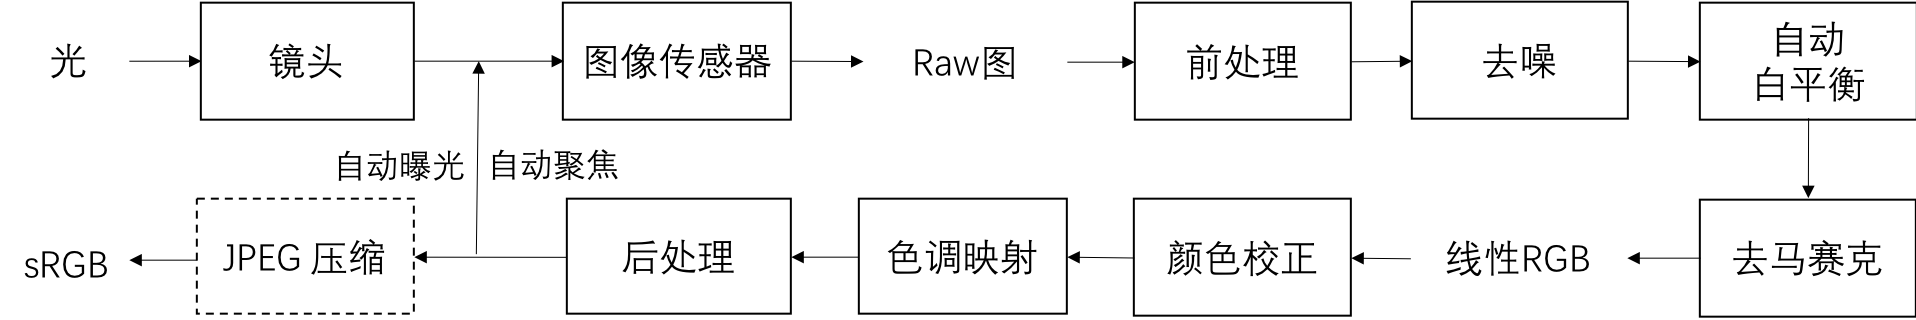
\includegraphics[width=0.9\textwidth]{Img/ISP_simple}
    \caption{简单ISP}
\end{figure}

图像是由许多像素组成,而图像语义分割(Semantic Image Segmentation)顾名思义就是将像素按照图像中表达语义含义的不同进行分组(Grouping)/分割(Segmentation),也就是可以根据图像内容(图像中的物体)进行像素级的分类。图像语义分割作为视觉人工智能中图像理解(Image Understanding)的重要一环,\upcite{li2000}不仅在军事和工业界的需求日益凸显,同时语义分割也是当下学术界的研究热点之一。图像语义分割可以说是图像理解的基石性技术,在自动驾驶系统(街景识别与理解)、自动目标识别、无人机军事侦查以及穿戴式设备应用中举足轻重。\upcite{Cong2011Sparse}

图像是由许多像素组成,而图像语义分割(Semantic Image Segmentation)顾名思义就是将像素按照图像中表达语义含义的不同进行分组(Grouping)/分割(Segmentation),也就是可以根据图像内容(图像中的物体)进行像素级的分类。图像语义分割作为视觉人工智能中图像理解(Image Understanding)的重要一环,\upcite{li2000}不仅在军事和工业界的需求日益凸显,同时语义分割也是当下学术界的研究热点之一。图像语义分割可以说是图像理解的基石性技术,在自动驾驶系统(街景识别与理解)、自动目标识别、无人机军事侦查以及穿戴式设备应用中举足轻重。\upcite{Cong2011Sparse}

图像是由许多像素组成,而图像语义分割(Semantic Image Segmentation)顾名思义就是将像素按照图像中表达语义含义的不同进行分组(Grouping)/分割(Segmentation),也就是可以根据图像内容(图像中的物体)进行像素级的分类。图像语义分割作为视觉人工智能中图像理解(Image Understanding)的重要一环,\upcite{li2000}不仅在军事和工业界的需求日益凸显,同时语义分割也是当下学术界的研究热点之一。图像语义分割可以说是图像理解的基石性技术,在自动驾驶系统(街景识别与理解)、自动目标识别、无人机军事侦查以及穿戴式设备应用中举足轻重。\upcite{Cong2011Sparse}

...


%%% ++++++++++++++++++++++++++++++++++++++++++++++++++++++++++++++++++++++++++++++++++
%   \include ?= \input + \clearpage
\clearpage
%%%%% --------------------------------------------------------------------------------
%%
%%%%******************************* Main Content *************************************
%%
%%% ++++++++++++++++++++++++++++++++++++++++++++++++++++++++++++++++++++++++++++++++++




\section{必要性}
\sectionnotes{(从国家军事战略、军事需求、服务作战和装备发展等方面阐述项目立项的迫切性。)}

	
   很多必要性……  



%%% ++++++++++++++++++++++++++++++++++++++++++++++++++++++++++++++++++++++++++++++++++
%
\printbibliography  % 打印参考文献
\clearpage
%%%%% --------------------------------------------------------------------------------
%%
%%%%******************************* Main Content *************************************
%%
%%% ++++++++++++++++++++++++++++++++++++++++++++++++++++++++++++++++++++++++++++++++++




\section{主要研究内容及应用前景分析}

\subsection{研究目标}
\sectionnotes{(简要说明项目的预期目标。)}


\subsection{研究内容}
\sectionnotes{(根据研究目标,列出具体研究条目,并简要论述针对的问题、采取的研究方法和技术手段、达到的目的。)}

	
\subsection{成果形式}
\sectionnotes{(详细说明项目预期的成果形式。比如,研究报告,含报告名称、份数;原理样机及技术文档,含样机的台/份数及相应的设计方案、设计图纸、使用维护手册等;软件系统及技术文档,含需求规格说明、软件设计、用户手册、软件测试或试用报告等。以及研究产生的模型、算法及数据等技术主题上的成果内容。)}




成果包含:
研究报告一份,包括研究产生的模型、算法和测试结果;
专利4-6个,包括核心技术形成的专利;
论文4-6篇,在国际顶级期刊和会议上发表论文。


\subsection{技术指标}
\sectionnotes{(根据研究内容,提出有针对性的、可考核的技术指标。研究类项目应明确研究任务要求、研究范围、项目具体成果及成果的主要技术贡献点;研制类项目应明确基本功能性能指标、自然环境适应性(气候、地理等)、战场环境适应性(电磁、伪装等)和勤务指标(人员、保障等)。)}


\subsection{应用前景分析}
\sectionnotes{(论述研究成果的推广应用方向,及产生的预期军事、社会效益等。)}


很多内容……


%%% ++++++++++++++++++++++++++++++++++++++++++++++++++++++++++++++++++++++++++++++++++
%
\clearpage
%%%%% --------------------------------------------------------------------------------
%%
%%%%******************************* Main Content *************************************
%%
%%% ++++++++++++++++++++++++++++++++++++++++++++++++++++++++++++++++++++++++++++++++++




\section{初步方案}

\subsection{总体方案}
\sectionnotes{(阐述本项目研究的总体思路、技术路线。)}



\subsection{主要技术分析}
\sectionnotes{(分析识别实现研究目标和技术方案的主要技术;针对每一项技术,论述拟采取的技术途径、解决办法。)}

\subsection{研制周期}
\subsubsection{项目周期:2年}
\sectionnotes{(项目研究的自然年数。)}

\subsubsection{进度安排}
\sectionnotes{(针对研究内容,逐项分解并明确具体进度安排,精确到月份。)}

2019.1-2019.5:项目总体设计。包括资料收集与分析,不同类型数据集的收集,实验环境的准备。形成项目的总体设计报告和详细的研究计划。

2019.6-2020.7:关键技术攻关。包括迁移学习算法和图卷积网络的研究。在国内外权威刊物发表学术论文,其中SCI论文 2篇,EI论文 2 篇。申请国家发明专利2-4项。

2020.8-2020.10: 进一步扩展。在之前研究的基础上,将图像语义分割扩展到实例级别上。在国内外权威刊物等发表学术论文,其中SCI 论文1篇,EI 论文2 篇。申请国家发明专利2-4项。

2020.11-2020.12:技术总结,文档撰写,项目结题验收。


\subsection{项目组组成}
\subsubsection{项目组负责人}
\sectionnotes{(简要介绍其相关领域科研经历,承担的重大科研任务,及获奖、专家情况。)}

\subsubsection{项目组}
\sectionnotes{(列表形式,简要描述项目组人员的学历、目前所从事的专业领域、在本项目中所承担的工作任务等。)}



%%% ++++++++++++++++++++++++++++++++++++++++++++++++++++++++++++++++++++++++++++++++++
%
\clearpage

%%%%% --------------------------------------------------------------------------------
%%
%%%%******************************* Main Content *************************************
%%
%%% ++++++++++++++++++++++++++++++++++++++++++++++++++++++++++++++++++++++++++++++++++


\section{经费概算和年度安排}


\subsection{军内科研项目经费预算表(单位:万元)}

\begin{table}[H]
	\centering
	\begin{tabular}{cccccc}
		\toprule
		序号 & 费用类型                          & 2020年 & 2021年 & 小计 & 备注 \\
		\midrule
		一   & 直接费                                                                          \\
		1    & 设备费                            & 10     & 10     & 20                        \\
		2    & 材料费                            & 2      & 2      & 4                         \\
		3    & 外部协作费                        & 15     & 15     & 30                        \\
		4    & 燃料动力费                        & 2      & 2      & 4                         \\
		5    & 会议/差旅/国际合作与交流费        & 10     & 10     & 20                        \\
		6    & 出版/文献/信息传播/知识产权事务费 & 6      & 6      & 12                        \\
		7    & 劳务费                            & 10     & 10     & 20                        \\
		8    & 专家咨询费                        & 2      & 2      & 4                         \\
		9    & 其他支出                          & 0                                           \\
		二   & 间接费                            &        &             & 10          \\
		三   & 合 计                             &        &             & 124         \\
		\bottomrule
	\end{tabular}
\end{table}




\subsection{项目直接经费预算明细表(单位:万元)}

\subsubsection{设备费}
\begin{table}[H]
	\centering
	\begin{tabular}{m{3cm} m{5cm} cccc}
		\toprule
		名  称           & 型号及详细配置          & 单价 & 数量 & 经费 & 备注
		\\
		\midrule
		深度学习处理平台 & Dell T630深度学习服务器 & 2    & 5    & 10
		\\
		并行计算显卡     & 华硕GTX1080             & 0.5  & 2    & 1
		\\
		合 计            &                         & 11   &
		                 &                                                     \\
		\bottomrule
	\end{tabular}
\end{table}

\subsubsection{材料费}
\begin{table}[H]
	\centering
	\begin{tabular}{m{3cm} m{3.5cm} cccc}
		\toprule
		名  称                   & 型号规格                                               & 单价         & 数量 & 经费 & 备注
		\\
		\midrule
		集中打印、复
		印费用                   & 集中性的复印、打印费用支付。                           & 0.5万/年*2年 & 0.5  & 2    & 1
		\\
		文件夹、文件袋等办公用品 & 具体包括:打印纸、墨盒、文件夹、文件袋等办公用品的购买 & 0.5          & 2    & 1           \\
		办公辅助用品和耗材       & 扫描仪、鼠标、键盘灯办公辅助用品的更新                 & 1            & 2    & 2           \\
		\\
		合 计                    &                                                        & 4            &
		                         &                                                                                            \\
		\bottomrule
	\end{tabular}
\end{table}

\subsubsection{外部协作费}
\begin{table}[H]
	\centering
	\begin{tabular}{m{3cm} m{7.5cm} cc}
		\toprule
		外协内容     & 外协单位     & 经费 & 备注 \\
		\midrule
		核心算法研究 & 西北工业大学 & 10   &      \\
		合 计        &              & 10          \\
		\bottomrule
	\end{tabular}
\end{table}

\subsubsection{燃料动力费}

\begin{table}[H]
	\centering
	\begin{tabular}{m{3cm} m{7.5cm} cc}
		\toprule
		项目           & 简要内容                                                               & 经费 & 备注 \\
		\midrule
		水电、空调费用 & 主要用于实验室测试过程所需交纳的水电费、空调费,每年2万元,两年4万元。 & 4    &      \\
		合 计          &                                                                        & 4           \\
		\bottomrule
	\end{tabular}
\end{table}

\subsubsection{会议/差旅/国际合作与交流费}
\begin{table}[H]
	\centering
	\begin{tabular}{m{3cm} m{7.5cm} cc}
		\toprule
		项目     & 简要内容                                                                                                         & 经费 & 备注 \\
		\midrule
		出差     & 主要用于项目研究过程中调研、学术交流、现场实施等所产生的差旅费,按照2年36人/次,每人/次约5000元计算,小计18万元; & 18   &      \\
		国际会议 & 期间拟出国参加2次学术会议,每次2人,每次出境时间4-6天,每人/次预算2万元,小计8万元;                              & 8    &      \\
		邀请专家 & 邀请境内外专家来访2人/次,每次预算2万元,小计4万元。                                                             & 4    &      \\
		合 计    &                                                                                                                  & 30          \\
		\bottomrule
	\end{tabular}
\end{table}

\subsubsection{出版/文献/信息传播/知识产权事务费费}
\begin{table}[H]
	\centering
	\begin{tabular}{m{3cm} m{7.5cm} cc}
		\toprule
		项目           & 简要内容                                               & 经费 & 备注 \\
		\midrule
		专利           & 请国家发明专利6个,申请专利费0.5万/个,小计3万元;     & 3    &      \\
		论文投稿和发表 & 发表学术论文10篇,审稿费、版面费3000元/篇,小计3万元; & 3    &      \\
		专著出版       & 出版专著1部,小计5万元。                               & 5    &      \\
		合 计          &                                                        & 11          \\
		\bottomrule
	\end{tabular}
\end{table}

\subsubsection{劳务费}
\begin{table}[H]
	\centering
	\begin{tabular}{m{3cm} m{7.5cm} cc}
		\toprule
		项目       & 简要内容                                                       & 经费 & 备注 \\
		\midrule
		研究生补助 & 没有工资性收入的在校研究生2人,每人每年补助1万(2年),小计4万 & 4    &      \\
		外聘人员   & 聘用软件工程师1人,年工资8万(2年),小计16万元                & 16   &      \\
		合 计      &                                                                & 20          \\
		\bottomrule
	\end{tabular}
\end{table}

\subsubsection{专家咨询费}
\begin{table}[H]
	\centering
	\begin{tabular}{m{3cm} m{7.5cm} cc}
		\toprule
		项目     & 简要内容                                                                                                  & 经费 & 备注 \\
		\midrule
		专家咨询 & 邀请国内专家对算法设计与实现方案进行评审4次,每次5人,按照学校有关规定,每次支付标准为2000元。该项共计4万 & 4    &      \\
		合 计    &                                                                                                           & 4           \\
		\bottomrule
	\end{tabular}
\end{table}

\subsubsection{其他支出}
\begin{table}[H]
	\centering
	\begin{tabular}{m{3cm} m{7.5cm} cc}
		\toprule
		项目       & 简要内容                       & 经费 & 备注 \\
		\midrule
		通讯邮寄费 & 因项目沟通、物资邮寄产生的费用 & 1    &      \\
		合 计      &                                & 1           \\
		\bottomrule
	\end{tabular}
\end{table}





%%% ++++++++++++++++++++++++++++++++++++++++++++++++++++++++++++++++++++++++++++++++++
%
\clearpage

%%%%% --------------------------------------------------------------------------------
%%
%%%%******************************* Main Content *************************************
%%
%%% ++++++++++++++++++++++++++++++++++++++++++++++++++++++++++++++++++++++++++++++++++


\section{可行性及风险分析}
\subsection{承研单位科研概况}
\sectionnotes{(简要描述承研单位的职能任务、主要研究方向,以及在本项目研究相关领域所承担的重大任务情况。)}


\subsection{科研保障条件}
\sectionnotes{(简要描述可用于本项目研究的已有科研条件手段建设、运用情况,以及项目组开展过的相关领域科研、人员保障情况。)}


\subsection{技术储备情况}
\sectionnotes{(简要描述承担单位及项目组在本项目领域有关调研分析、实验/试验、技术研究、前沿技术跟踪、模型数据积累等技术储备情况。)}


\subsection{风险分析}
\sectionnotes{(本项目研究在技术突破、时间进度安排、人力资源保障、条件手段应用、经费开支保障等方面所存在的风险及规避措施。)}

本项目研究课题组有一定的研究基础,在时间进度安排、人力资源保障和经费开支等方面风险可控。
%%% ++++++++++++++++++++++++++++++++++++++++++++++++++++++++++++++++++++++++++++++++++
%
\clearpage
%%%%% --------------------------------------------------------------------------------
%%
%%%%******************************* Main Content *************************************
%%
%%% ++++++++++++++++++++++++++++++++++++++++++++++++++++++++++++++++++++++++++++++++++




\section{有关部门意见}

\def\arraystretch{7.0}
{\kai
\begin{tabular}{|p{16.1cm}|}
	 \hline
\makecell[l]{项目申报单位意见 \\
	\\
	\\
	\\
	\\
	\quad\quad\quad\quad\quad\quad\quad\quad\quad\quad\quad\quad\quad\quad\quad\quad\quad\quad\quad\quad\quad\quad\quad\quad\quad\quad\quad\quad\quad 单位盖章 \\
	\quad\quad\quad\quad\quad\quad\quad\quad\quad\quad\quad\quad\quad\quad\quad\quad\quad\quad\quad\quad\quad\quad\quad\quad\quad\quad\quad\quad\quad  年   \quad 月  \quad  日 \\
	\\ \\ 
} \\ \hline

\makecell[l]{上级主管部门审核意见 \\
	\\
	\\
	\\
	\\
	\quad\quad\quad\quad\quad\quad\quad\quad\quad\quad\quad\quad\quad\quad\quad\quad\quad\quad\quad\quad\quad\quad\quad\quad\quad\quad\quad\quad\quad 单位盖章 \\
	\quad\quad\quad\quad\quad\quad\quad\quad\quad\quad\quad\quad\quad\quad\quad\quad\quad\quad\quad\quad\quad\quad\quad\quad\quad\quad\quad\quad\quad  年   \quad 月  \quad  日 \\
	\\ \\
} \\ \hline
\makecell[l]{科研管理部门审核意见 \\
	\\
	\\
	\\
	\\
	\quad\quad\quad\quad\quad\quad\quad\quad\quad\quad\quad\quad\quad\quad\quad\quad\quad\quad\quad\quad\quad\quad\quad\quad\quad\quad\quad\quad\quad 单位盖章 \\
	\quad\quad\quad\quad\quad\quad\quad\quad\quad\quad\quad\quad\quad\quad\quad\quad\quad\quad\quad\quad\quad\quad\quad\quad\quad\quad\quad\quad\quad  年   \quad 月  \quad  日 \\
	\\ \\ 
} \\ \hline
\end{tabular}
}

%%% ++++++++++++++++++++++++++++++++++++++++++++++++++++++++++++++++++++++++++++++++++
%
\clearpage

\end{document}
%%%%% --------------------------------------------------------------------------------
